\documentclass[11pt,a4paper]{article}

\usepackage[utf8]{inputenc}
\usepackage[T1]{fontenc}
\usepackage[brazilian]{babel}
\usepackage{geometry}
\usepackage{graphicx}
\usepackage{booktabs}
\usepackage{float}
\usepackage{enumitem}
\usepackage{amsmath}
\usepackage{xcolor}
\usepackage{fancyhdr}
\usepackage{setspace}
\usepackage{hyperref}
\usepackage{tcolorbox}
\usepackage{subcaption}
\usepackage{pdflscape}

\geometry{left=2.5cm,right=2.5cm,top=2.5cm,bottom=2.5cm}
\setlength{\parindent}{0pt}
\setlength{\parskip}{0.55em}
\onehalfspacing

\tcbuselibrary{skins,breakable}
\newtcolorbox{instrucao}[1][]{colback=blue!5,colframe=blue!40!black,
  fonttitle=\bfseries, title=#1, breakable}
\newtcolorbox{atencao}[1][]{colback=orange!10,colframe=orange!60!black,
  fonttitle=\bfseries, title=#1, breakable}

\pagestyle{fancy}
\fancyhf{}
\fancyhead[L]{\small FGA0092 -- Princípios de Comunicação para Engenharia}
\fancyhead[R]{\small Enunciado -- Prática 06}
\fancyfoot[C]{\small\thepage}
\renewcommand{\headrulewidth}{0.4pt}

\begin{document}

\begin{center}
  
\includegraphics[width=0.18\textwidth]{../../figures_global/unb.png}\\[0.5cm]
  {\large\textbf{Universidade de Brasília (UnB) -- FCTE}}\\[0.2cm]
  {\normalsize FGA0092 -- Princípios de Comunicação para Engenharia}\\[0.4cm]
  \rule{14cm}{0.8pt}\\[0.3cm]
  {\LARGE\textbf{Prática 06}}\\[0.15cm]
  {\Large\textbf{Demodulação FM: Detector de Inclinação e Discriminador Balanceado}}\\[0.3cm]
  \rule{14cm}{0.8pt}
\end{center}

\vspace{0.3cm}
\textbf{Duração:} 50 minutos \hfill
\textbf{Software:} GNU Radio Companion $\geq$ 3.10 \hfill
\textbf{Semestre:} 2026/2

\textbf{Pré-requisito:} Prática 05, com o transmissor \texttt{Signal Source} $\to$
\texttt{Frequency Mod} e o discriminador \texttt{Quadrature Demod}.

\bigskip

% ======================================================
\section{Objetivos}

\begin{itemize}
  \item Construir um detector de inclinação e um discriminador balanceado a
    partir de filtros passa-faixa e detectores de envoltória.
  \item Medir a amplitude e as harmônicas da saída de cada demodulador e
    comparar com o discriminador de quadratura da Prática 05.
  \item Medir a relação entre o tom e o piso de ruído na saída de cada
    demodulador em função da relação portadora-ruído na entrada.
\end{itemize}

% ======================================================
\section{Fundamentos teóricos}

O sinal FM em banda base complexa tem frequência instantânea
$f_i(t) = \Delta f\,m(t)$, com $m(t)=\cos(2\pi f_m t)$; ela percorre o
intervalo $[-\Delta f, \Delta f]$.

\textbf{Detector de inclinação.} O filtro \texttt{bpf\_pos} deixa passar de
$\Delta f$ a $5\Delta f$ com transição de largura $4\Delta f$ em torno de cada
borda. A borda inferior é uma rampa que sobe de $f=-\Delta f$ até
$f=3\Delta f$, e $f_i(t)$ percorre a metade de baixo dessa rampa, onde ela é
curva. A envoltória na saída do filtro segue $|H_+(f_i)|$:
\begin{equation}
  v_+(t) = |H_+(f_i(t))| = K_0 + K_1 m(t) + K_2 m^2(t) + K_3 m^3(t) + \cdots
  \label{eq:vpos}
\end{equation}
Como $m^2 = \tfrac12 + \tfrac12\cos 2\omega_m t$ e
$m^3 = \tfrac34\cos\omega_m t + \tfrac14\cos 3\omega_m t$, a saída tem nível CC,
removido pelo \texttt{DC Blocker}, e harmônicas em $2f_m$ e $3f_m$.

\textbf{Discriminador balanceado.} O filtro \texttt{bpf\_neg} é o espelho de
\texttt{bpf\_pos} em torno de $0$\,Hz, de modo que $|H_-(f)| = |H_+(-f)|$ e
\begin{equation}
  v_-(t) = K_0 - K_1 m(t) + K_2 m^2(t) - K_3 m^3(t) + \cdots
\end{equation}
A diferença cancela os termos de ordem par e dobra os de ordem ímpar:
\begin{equation}
  v_+(t) - v_-(t) = 2K_1 m(t) + 2K_3 m^3(t) + \cdots
  \label{eq:balanced}
\end{equation}
Portanto a amplitude da fundamental dobra, $+6{,}02$\,dB, a harmônica em $2f_m$
desaparece e a harmônica em $3f_m$ mantém o mesmo nível relativo.

\textbf{Distorção harmônica.} Com $H_k$ o nível em dB da harmônica $k$ lido no
espectro,
\begin{equation}
  \mathrm{THD} = 10\log_{10}\!\Big(10^{(H_2-H_1)/10} + 10^{(H_3-H_1)/10}\Big)\ \text{dB},
  \qquad
  \mathrm{THD}_{\%} = 100\cdot 10^{\mathrm{THD}/20}.
  \label{eq:thd}
\end{equation}

\textbf{Ruído.} O \texttt{Noise Source} complexo com amplitude $\sigma$ tem
potência $\sigma^2$ espalhada em \texttt{samp\_rate}. Dentro da banda de Carson
$B_C = 2(\Delta f + f_m)$, a relação portadora-ruído do sinal de amplitude 1 é
\begin{equation}
  \frac{C}{N} = 10\log_{10}\frac{1}{\sigma^2\,B_C/\texttt{samp\_rate}}\ \text{dB}.
  \label{eq:cn}
\end{equation}
Na saída, a qualidade é medida pela relação tom-piso
\begin{equation}
  R = L(f_m) - L(2{,}5\ \text{kHz})\ \text{dB},
  \label{eq:r}
\end{equation}
diferença entre o nível do tom e o nível do piso de ruído em $2{,}5$\,kHz, entre
a 2.ª e a 3.ª harmônicas.

% ======================================================
\section{Materiais e blocos GNU Radio}

\begin{table}[H]
  \centering\small
  \begin{tabular}{l l l}
    \toprule
    \textbf{Bloco GRC} & \textbf{Localização} & \textbf{Função} \\
    \midrule
    \texttt{Variable}, \texttt{QT GUI Range} & Variables, GUI Widgets & Parâmetros e sliders \\
    \texttt{Import}            & Misc                 & \texttt{import math} \\
    \texttt{Signal Source}     & Waveform Generators  & Mensagem $m(t)$ \\
    \texttt{Frequency Mod}     & Modulators           & Modulador FM \\
    \texttt{Throttle}          & Misc                 & Limita a taxa de execução \\
    \texttt{Noise Source}      & Waveform Generators  & Ruído gaussiano \\
    \texttt{Add}               & Math Operators       & Soma do ruído ao sinal FM \\
    \texttt{Band Pass Filter}  & Filters              & Filtros de inclinação \\
    \texttt{Complex to Mag}    & Type Converters      & Detector de envoltória \\
    \texttt{Subtract}          & Math Operators       & Subtração balanceada \\
    \texttt{DC Blocker}        & Filters              & Remoção do nível CC \\
    \texttt{Low Pass Filter}   & Filters              & Filtro de áudio e decimação \\
    \texttt{Quadrature Demod}  & Modulators           & Referência da Prática 05 \\
    \texttt{Keep 1 in N}       & Stream Operators     & Mensagem na taxa de áudio \\
    \texttt{QT GUI Frequency Sink}, \texttt{Time Sink} & Instrumentation & Medições \\
    \bottomrule
  \end{tabular}
  \caption{Blocos utilizados na Prática 06.}
\end{table}

\begin{landscape}
\begin{figure}[p]
  \centering
  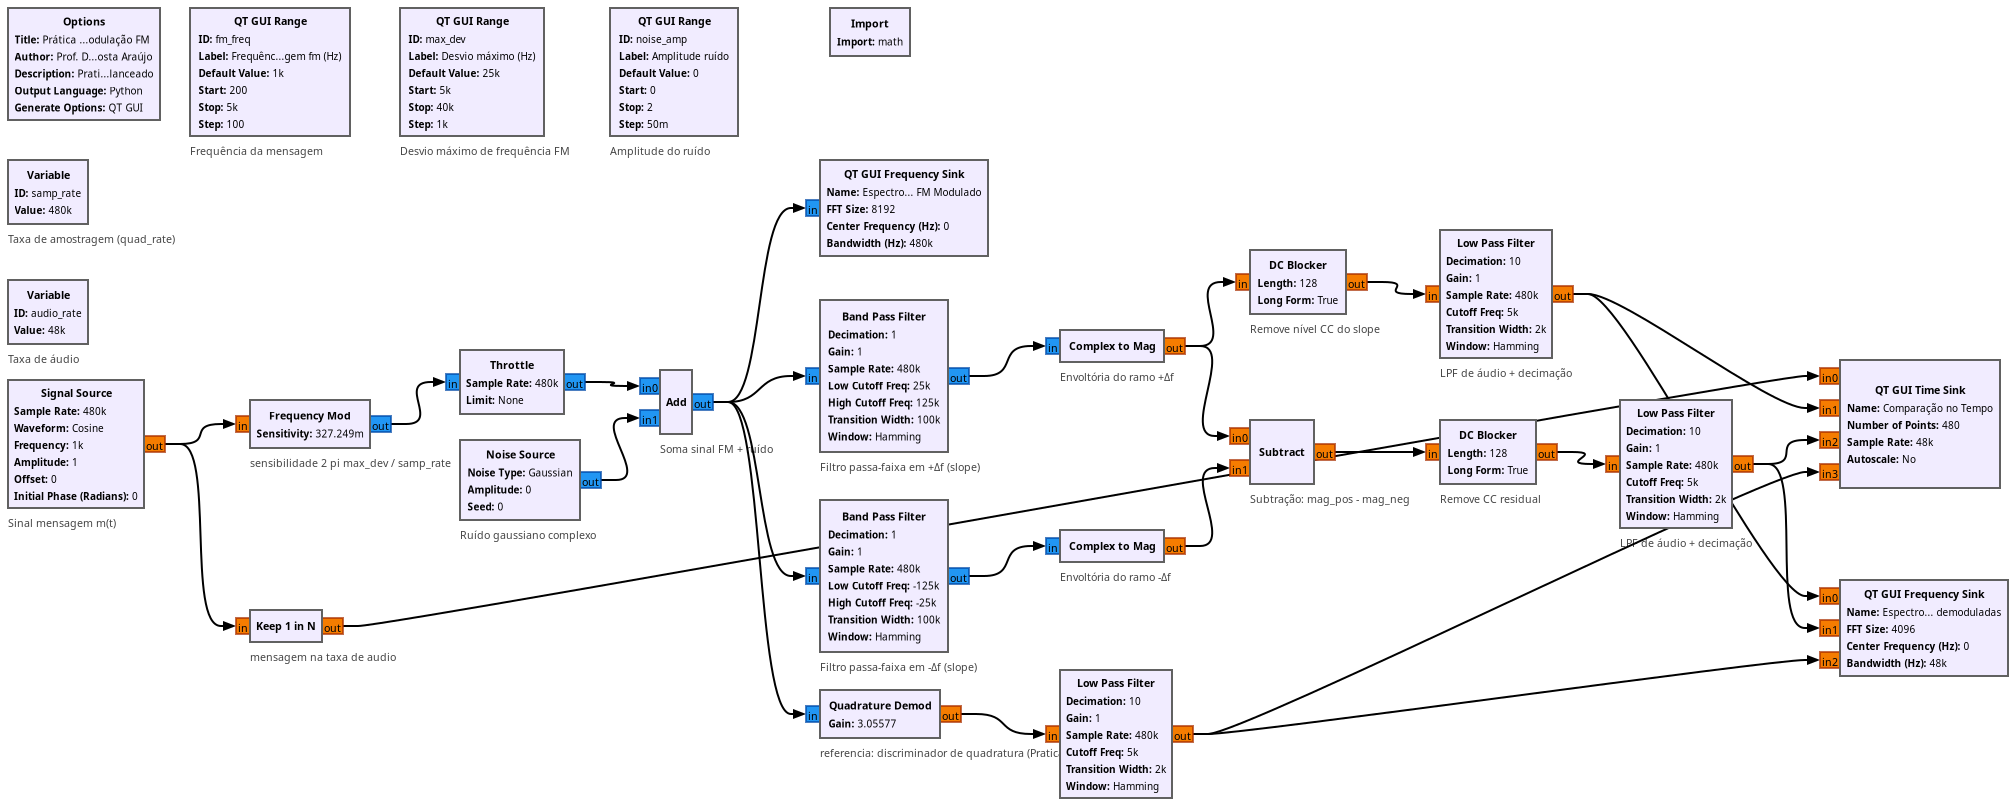
\includegraphics[width=\linewidth]{figuras/flowgraph.png}
  \caption{Flowgraph completo da Prática 06, como aparece no GNU Radio Companion.}
  \label{fig:flowgraph}
\end{figure}
\end{landscape}

\begin{figure}[H]
  \centering
  \begin{subfigure}{0.49\textwidth}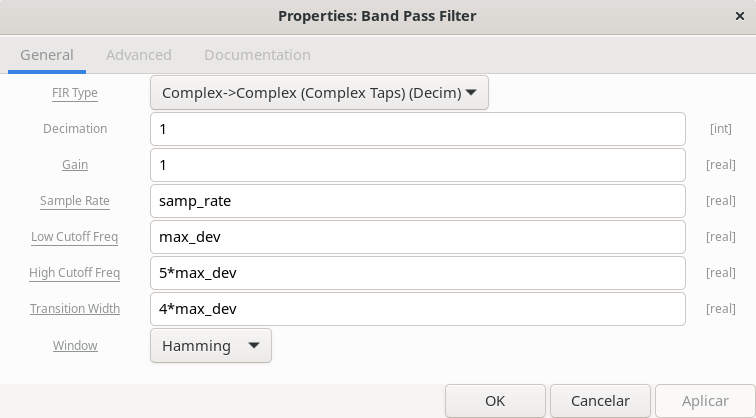
\includegraphics[width=\textwidth]{figuras/bloco_bpf_pos.png}\caption{\texttt{bpf\_pos}}\end{subfigure}
  \begin{subfigure}{0.49\textwidth}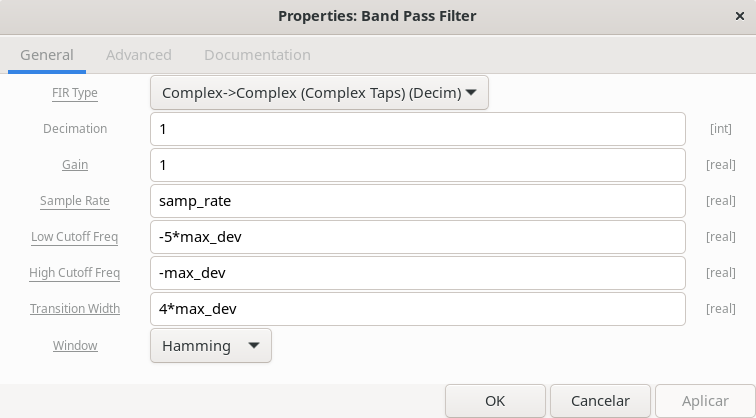
\includegraphics[width=\textwidth]{figuras/bloco_bpf_neg.png}\caption{\texttt{bpf\_neg}}\end{subfigure}\\[4pt]
  \begin{subfigure}{0.49\textwidth}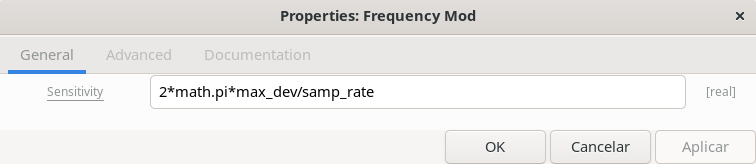
\includegraphics[width=\textwidth]{figuras/bloco_fm_mod.png}\caption{Frequency Mod}\end{subfigure}
  \begin{subfigure}{0.49\textwidth}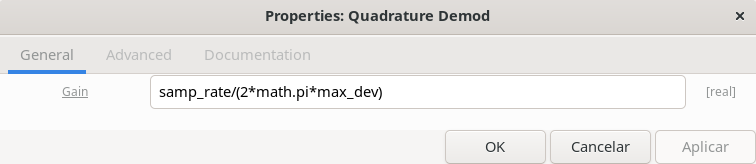
\includegraphics[width=\textwidth]{figuras/bloco_quad_demod.png}\caption{Quadrature Demod, referência}\end{subfigure}\\[4pt]
  \begin{subfigure}{0.49\textwidth}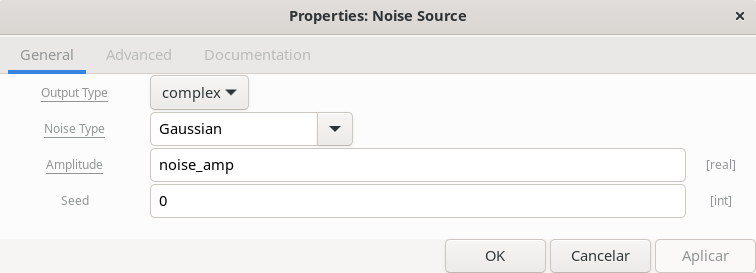
\includegraphics[width=\textwidth]{figuras/bloco_src_noise.png}\caption{Noise Source}\end{subfigure}
  \begin{subfigure}{0.49\textwidth}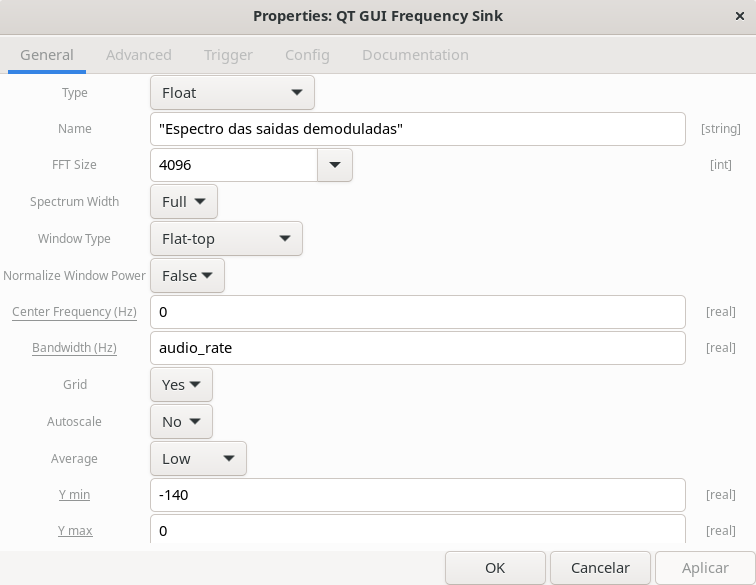
\includegraphics[width=\textwidth]{figuras/bloco_freq_sink_demod.png}\caption{Frequency Sink das saídas}\end{subfigure}
  \caption{Parâmetros dos blocos principais, capturados do GNU Radio Companion.
    Os dois \texttt{Band Pass Filter} usam o tipo \textit{Complex$\to$Complex (Complex Taps)}.}
  \label{fig:blocos}
\end{figure}

% ======================================================
\section{Roteiro de montagem e execução (50 min)}

\subsection*{Parâmetros}

\begin{center}\small
\begin{tabular}{l l}
  \toprule
  \texttt{samp\_rate}, \texttt{audio\_rate} & $480\,000$\,Hz, $48\,000$\,Hz \\
  \texttt{fm\_freq} & $200$ a $5\,000$\,Hz, passo $100$, padrão $1\,000$ \\
  \texttt{max\_dev} & $5\,000$ a $34\,000$\,Hz, passo $1\,000$, padrão $25\,000$ \\
  \texttt{noise\_amp} & $0$ a $2$, passo $0{,}05$, padrão $0$ \\
  Frequency Mod, \textit{Sensitivity} & \texttt{2*math.pi*max\_dev/samp\_rate} \\
  \texttt{bpf\_pos} & corte \texttt{max\_dev} a \texttt{5*max\_dev}, transição \texttt{4*max\_dev}, Hamming \\
  \texttt{bpf\_neg} & corte \texttt{-5*max\_dev} a \texttt{-max\_dev}, transição \texttt{4*max\_dev}, Hamming \\
  DC Blocker & comprimento $128$, forma longa \\
  Low Pass Filter & corte $5$\,kHz, transição $2$\,kHz, decimação $10$ \\
  Quadrature Demod, \textit{Gain} & \texttt{samp\_rate/(2*math.pi*max\_dev)} \\
  Keep 1 in N & $N = 10$ \\
  Frequency Sink do sinal FM & complex, FFT $8\,192$, \textit{Flat-top}, eixo $-100$ a $10$\,dB \\
  Frequency Sink das saídas & float, $3$ entradas, FFT $4\,096$, \textit{Flat-top}, média $0{,}2$ \\
  Time Sink & float, $4$ entradas, $480$ pontos, $10$\,ms, eixo $\pm 1{,}2$ \\
  \bottomrule
\end{tabular}
\end{center}

\begin{atencao}[Atenção -- limite de \texttt{max\_dev}]
A borda superior de \texttt{bpf\_pos} fica em $5\,\Delta f$, e a transição de
largura $4\,\Delta f$ é centrada nela, de modo que a rampa de descida vai até
$7\,\Delta f$. Essa rampa precisa terminar abaixo de
$\texttt{samp\_rate}/2 = 240$\,kHz, senão ela se rebate para as frequências
negativas. Por isso o slider vai só até $34$\,kHz, que leva a rampa a
$238$\,kHz.
\end{atencao}

\begin{instrucao}[Leitura dos instrumentos]
No Frequency Sink das saídas, passe o mouse sobre o topo de cada componente para
ler o nível em dB. Use só diferenças entre níveis: elas não dependem da escala
do instrumento. No Time Sink, a amplitude é metade do valor pico a pico. As saídas de
inclinação e do balanceado ficam abaixo de $0{,}2$: ative o \textit{Autoscale}
no menu do botão direito para lê-las.
\end{instrucao}

\subsection*{Etapa 1 -- Transmissor (0--6 min)}

\begin{instrucao}[Reaproveitar o transmissor da Prática 05]
\begin{enumerate}[label=\arabic*.]
  \item Monte \texttt{Signal Source} $\to$ \texttt{Frequency Mod} $\to$
    \texttt{Throttle} $\to$ \texttt{Add} com o \texttt{Noise Source} na segunda
    entrada, com os parâmetros acima.
  \item Ligue a saída do \texttt{Add} ao Frequency Sink do sinal FM e confira
    que o espectro ocupa cerca de $\pm 26$\,kHz, metade de
    $B_C = 2(25 + 1) = 52$\,kHz.
\end{enumerate}
\end{instrucao}

\subsection*{Etapa 2 -- Detector de inclinação (6--18 min)}

\begin{instrucao}[Ramo \texttt{bpf\_pos}]
\begin{enumerate}[label=\arabic*.]
  \item Monte \texttt{Add} $\to$ \texttt{bpf\_pos} $\to$ \texttt{Complex to Mag}
    $\to$ \texttt{DC Blocker} $\to$ \texttt{Low Pass Filter} e ligue a saída ao
    canal 1 do Time Sink e à entrada 0 do Frequency Sink das saídas.
  \item Ligue \texttt{Signal Source} $\to$ \texttt{Keep 1 in N} ao canal 0 do
    Time Sink, para comparar com a mensagem.
  \item Com $f_m = 1$\,kHz, $\Delta f = 25$\,kHz e sem ruído, meça a amplitude
    da saída no Time Sink e os níveis $H_1$, $H_2$ e $H_3$ em $1$, $2$ e
    $3$\,kHz. Preencha a linha \textit{inclinação} da Tabela~\ref{tab:harm}.
\end{enumerate}
\end{instrucao}

\subsection*{Etapa 3 -- Discriminador balanceado (18--28 min)}

\begin{instrucao}[Ramo \texttt{bpf\_neg} e subtração]
\begin{enumerate}[label=\arabic*.]
  \item Monte \texttt{Add} $\to$ \texttt{bpf\_neg} $\to$ \texttt{Complex to Mag}.
  \item Subtraia: envoltória de \texttt{bpf\_pos} na entrada 0 do \texttt{Subtract}
    e envoltória de \texttt{bpf\_neg} na entrada 1. Depois
    \texttt{DC Blocker} $\to$ \texttt{Low Pass Filter} $\to$ canal 2 do Time Sink
    e entrada 1 do Frequency Sink das saídas.
  \item Meça amplitude, $H_1$, $H_2$ e $H_3$ e preencha a linha
    \textit{balanceado}.
\end{enumerate}
\end{instrucao}

\subsection*{Etapa 4 -- Referência de quadratura (28--34 min)}

\begin{instrucao}[Discriminador da Prática 05]
\begin{enumerate}[label=\arabic*.]
  \item Monte \texttt{Add} $\to$ \texttt{Quadrature Demod} $\to$
    \texttt{Low Pass Filter} $\to$ canal 3 do Time Sink e entrada 2 do Frequency
    Sink das saídas. Com o ganho da tabela de parâmetros, a saída é $m(t)$.
  \item Meça amplitude e níveis e preencha a linha \textit{quadratura}. Se uma
    harmônica não aparecer acima do piso, registre ``abaixo do piso''.
\end{enumerate}
\end{instrucao}

\begin{table}[H]
  \centering
  \begin{tabular}{l c c c c c}
    \toprule
    Saída & Amplitude & $H_2-H_1$ (dB) & $H_3-H_1$ (dB) & THD (dB) & THD (\%) \\
    \midrule
    Inclinação & & & & & \\
    Balanceado & & & & & \\
    Quadratura & & & & & \\
    \bottomrule
  \end{tabular}
  \caption{Saídas sem ruído, $f_m = 1$\,kHz, $\Delta f = 25$\,kHz. THD pela
    equação~\eqref{eq:thd}.}
  \label{tab:harm}
\end{table}

\subsection*{Etapa 5 -- Ruído (34--48 min)}

\begin{instrucao}[Relação tom-piso em função de \texttt{noise\_amp}]
\begin{enumerate}[label=\arabic*.]
  \item Para cada valor de \texttt{noise\_amp} da Tabela~\ref{tab:ruido},
    espere a média do Frequency Sink estabilizar, cerca de $3$\,s.
  \item Em cada uma das três saídas, leia o nível do tom em $1$\,kHz e o nível
    do piso em $2{,}5$\,kHz e calcule $R$ pela equação~\eqref{eq:r}.
  \item Calcule $C/N$ pela equação~\eqref{eq:cn}.
\end{enumerate}
\end{instrucao}

\begin{table}[H]
  \centering\small
  \begin{tabular}{c c c c c}
    \toprule
    \texttt{noise\_amp} & $C/N$ em $B_C$ (dB) & $R$ inclinação (dB) & $R$ balanceado (dB) & $R$ quadratura (dB) \\
    \midrule
    0,1 & & & & \\
    0,3 & & & & \\
    0,5 & & & & \\
    0,7 & & & & \\
    1,0 & & & & \\
    1,5 & & & & \\
    \bottomrule
  \end{tabular}
  \caption{Relação tom-piso nas três saídas, $f_m = 1$\,kHz, $\Delta f = 25$\,kHz.}
  \label{tab:ruido}
\end{table}

\subsection*{Síntese (48--50 min)}

Confira se as duas tabelas estão completas, com unidades.

% ======================================================
\section{Perguntas para o relatório}

Todas as respostas devem ser numéricas, com as contas mostradas.

\begin{enumerate}[label=\textbf{Q\arabic*.}, leftmargin=*]

  \item Calcule a razão entre as amplitudes do balanceado e da inclinação, em
    vezes e em dB, e compare com o fator $2$, ou $6{,}02$\,dB, da
    equação~\eqref{eq:balanced}.

  \item Quantos dB o discriminador balanceado reduziu a harmônica em $2f_m$ em
    relação ao detector de inclinação? E quanto mudou $H_3 - H_1$?

  \item Calcule a THD de cada saída em dB e em porcentagem. Por que fator a THD
    do balanceado é menor que a do detector de inclinação?

  \item Preencha a coluna $C/N$ da Tabela~\ref{tab:ruido}. Entre
    \texttt{noise\_amp} $= 0{,}3$ e $0{,}7$, quantos dB caiu $C/N$ e quantos dB
    caiu $R$ em cada uma das três saídas?

  \item Para cada saída, calcule a queda de $R$ por dB de queda de $C/N$ em
    cada intervalo da Tabela~\ref{tab:ruido}. Em que faixa de $C/N$ a saída de
    quadratura passa a cair mais de $3$\,dB por dB? Esse é o limiar do FM.

  \item Quanto a quadratura supera o balanceado em $R$ com
    \texttt{noise\_amp} $= 0{,}1$ e com \texttt{noise\_amp} $= 1{,}5$?

\end{enumerate}

% ======================================================
\section*{Entregáveis}

Relatório em PDF contendo:
\begin{itemize}
  \item As Tabelas~\ref{tab:harm} e~\ref{tab:ruido} preenchidas.
  \item Captura do Time Sink e do Frequency Sink das saídas sem ruído e com
    \texttt{noise\_amp} $= 1{,}0$.
  \item Respostas às perguntas Q1 a Q6.
\end{itemize}

\end{document}
